% =====================================================================
%  ElderCare Insight — Submission Report
%  Group Assignment #1 — Mini Data Warehouse & Analytics Dashboard
%
%  Build:  cd 06_Report && latexmk -xelatex -outdir=build eldercare_report.tex
%          cp build/eldercare_report.pdf .
%
%  XeLaTeX only (fontspec).
%
%  This is the SUBMISSION report (10-15 pages), not the design document.
%  eldercare_dw_design.tex is the pre-implementation design spec and is
%  deliberately left untouched; this report is written against what was
%  actually built and measured.
%
%  Language: English. The design document and every README are Thai, per
%  project convention, but the report was written in English by decision of
%  the group. A useful side effect: no Thai glyph appears in this source, so
%  the report needs no Thai font and builds on Windows/MiKTeX and Fedora/TeX
%  Live alike. Thai text survives only inside the dashboard screenshots,
%  which are bitmaps; section 7 translates the labels visible in them.
%
%  Fonts are taken from inside the TeX distribution (TeX Gyre + DejaVu), not
%  from the operating system, so no font install is required on either box.
%
%  Every figure is referenced in place from ../04_Dashboard/ rather than
%  copied here, so the images cannot drift from make_figures.py output.
%
%  Provenance of the numbers in this report:
%    - warehouse row counts, coverage, additivity gap  <- eldercare.duckdb,
%      queried read-only on 22 August 2569
%    - business answers and their tables               <- 06_Report/BQ_answers.md
%      (all produced by 04_Dashboard/queries_mpl.py)
%    - data quality counts                             <- etl_run_log table
% =====================================================================

\documentclass[11pt,a4paper]{article}

% ---------------------------------------------------------------------
%  FONTS — shipped with the TeX distribution, so nothing has to be
%  installed system-wide. Laksaman/Garuda (used by the Thai design
%  document) are NOT available on every machine in the group.
% ---------------------------------------------------------------------
\usepackage{fontspec}
\setmainfont{texgyrepagella}[
  Extension=.otf, UprightFont=*-regular, BoldFont=*-bold,
  ItalicFont=*-italic, BoldItalicFont=*-bolditalic]
\setsansfont{texgyreheros}[
  Extension=.otf, UprightFont=*-regular, BoldFont=*-bold,
  ItalicFont=*-italic, BoldItalicFont=*-bolditalic]
\setmonofont{DejaVuSansMono}[
  Extension=.ttf, BoldFont=*-Bold, Scale=0.82]

\newcommand{\sansall}{\sffamily}
\emergencystretch=2.2em

% ---------------------------------------------------------------------
%  LAYOUT
% ---------------------------------------------------------------------
\usepackage[a4paper,margin=2.0cm,top=2.1cm,bottom=1.9cm,headsep=10pt]{geometry}
\usepackage{amsmath,amssymb}
\usepackage{graphicx}
% Reference the dashboard's own output directly — copying the images here
% would let the report drift from what make_figures.py last produced.
\graphicspath{{figures/}{../04_Dashboard/}{../04_Dashboard/screenshots/}}
\usepackage{booktabs}
\usepackage{array}
\usepackage{longtable}
\usepackage{xcolor}
% [strings] so snake_case survives inside \includegraphics file names too,
% not only in body text. Plain \usepackage{underscore} breaks graphics paths.
\usepackage[strings]{underscore}
\usepackage{tikz}
\usetikzlibrary{arrows.meta,positioning,calc,shapes.geometric,shapes.misc,
                shapes.multipart,fit,backgrounds}
\usepackage[most]{tcolorbox}
\usepackage[font=small,labelfont=bf,width=0.95\textwidth]{caption}
\usepackage{fancyhdr}
\usepackage{enumitem}
\usepackage{titlesec}
\usepackage{float}
\usepackage{adjustbox}
\usepackage{microtype}
\usepackage[colorlinks=true,allcolors=src,breaklinks=true,
            bookmarksnumbered=true]{hyperref}

\linespread{1.0}
\setlength{\parskip}{0.26em}
\setlength{\parindent}{0pt}

% Floats are allowed to move. Pinning everything with [H] left half-empty
% pages wherever a figure could not fit in the remaining space, which is how
% the first draft reached 20 pages. These fractions let a float share a page
% with more text and discourage near-empty float pages.
\renewcommand{\topfraction}{0.92}
\renewcommand{\bottomfraction}{0.85}
\renewcommand{\textfraction}{0.06}
\renewcommand{\floatpagefraction}{0.75}
\setlength{\textfloatsep}{10pt plus 2pt minus 2pt}
\setlength{\intextsep}{9pt plus 2pt minus 2pt}

% ---------------------------------------------------------------------
%  COLOUR — the four pipeline stages, same palette as the design document
%  and the dashboard charts. Base is Okabe-Ito (colour-blind safe).
% ---------------------------------------------------------------------
\definecolor{src}{HTML}{0072B2}    % stage 1 — sources (blue)
\definecolor{etl}{HTML}{D55E00}    % stage 2 — ETL (orange)
\definecolor{dw}{HTML}{009E73}     % stage 3 — warehouse (green)
\definecolor{dash}{HTML}{7B5EA7}   % stage 4 — dashboard (purple)

\definecolor{ink}{HTML}{1A2733}
\definecolor{muted}{HTML}{5B6B7A}
\definecolor{rule}{HTML}{C9D2DB}
\definecolor{wash}{HTML}{F1F6FA}
\definecolor{warnwash}{HTML}{FDF3E7}
\definecolor{goodwash}{HTML}{E9F4F0}
\definecolor{badwash}{HTML}{FBEDED}
\definecolor{bad}{HTML}{B3261E}

% ---------------------------------------------------------------------
%  HEADINGS
% ---------------------------------------------------------------------
\titleformat{\section}
  {\sansall\large\bfseries\color{src!88!black}}{\thesection}{0.6em}{}
\titleformat{\subsection}
  {\sansall\normalsize\bfseries\color{ink}}{\thesubsection}{0.5em}{}
\titlespacing*{\section}{0pt}{1.3em}{0.5em}
\titlespacing*{\subsection}{0pt}{0.9em}{0.3em}

\pagestyle{fancy}
\fancyhf{}
\renewcommand{\headrulewidth}{0.4pt}
\fancyhead[L]{\footnotesize\sansall\color{muted}ElderCare Insight — Mini DW \& Dashboard}
\fancyhead[R]{\footnotesize\sansall\color{muted}Group 01}
\fancyfoot[C]{\footnotesize\color{muted}\thepage}

\setlist[itemize]{itemsep=1pt,topsep=2pt,parsep=0pt,leftmargin=1.3em}
\setlist[enumerate]{itemsep=1pt,topsep=2pt,parsep=0pt,leftmargin=1.5em}

% ---------------------------------------------------------------------
%  CALLOUT BOXES — four fixed meanings. Project convention forbids a fifth.
%    keybox  (blue)   the point
%    warnbox (orange) a caution
%    goodbox (green)  something confirmed against real data
%    badbox  (red)    a mistake that is easy to make
% ---------------------------------------------------------------------
\tcbset{guidebox/.style={
  enhanced, breakable, boxrule=0pt, leftrule=2.5pt, arc=1pt,
  left=7pt, right=7pt, top=5pt, bottom=5pt,
  fonttitle=\sansall\bfseries\small, titlerule=0pt,
  toptitle=1pt, bottomtitle=1pt}}

\newtcolorbox{keybox}[1][]{guidebox, colback=wash, colframe=src,
  colbacktitle=wash, coltitle=src!85!black, #1}
\newtcolorbox{warnbox}[1][]{guidebox, colback=warnwash, colframe=etl,
  colbacktitle=warnwash, coltitle=etl!80!black, #1}
\newtcolorbox{goodbox}[1][]{guidebox, colback=goodwash, colframe=dw,
  colbacktitle=goodwash, coltitle=dw!65!black, #1}
\newtcolorbox{badbox}[1][]{guidebox, colback=badwash, colframe=bad,
  colbacktitle=badwash, coltitle=bad, #1}

% ---------------------------------------------------------------------
%  SEMANTIC MARKUP
% ---------------------------------------------------------------------
\newcommand{\code}[1]{\texttt{#1}}
\newcommand{\PK}{\textcolor{dw}{\textbf{PK}}}
\newcommand{\FK}{\textcolor{src}{\textbf{FK}}}
\newcommand{\DD}{\textcolor{muted}{\textbf{DD}}}

% ---------------------------------------------------------------------
%  DIAGRAM GRAMMAR — same styles as the design document
% ---------------------------------------------------------------------
\tikzset{
  blk/.style={draw=rule, line width=0.6pt, rounded corners=2.5pt,
              fill=wash, minimum height=8mm, inner xsep=5pt, inner ysep=4pt,
              align=center, font=\sansall\footnotesize},
  srcb/.style={blk, fill=src!8,  draw=src!45},
  etlb/.style={blk, fill=etl!8,  draw=etl!45},
  dwb/.style={blk,  fill=dw!8,   draw=dw!45},
  dashb/.style={blk,fill=dash!8, draw=dash!45},
  ar/.style={-{Stealth[length=2.2mm,width=1.8mm]}, line width=0.7pt, draw=muted},
  lbl/.style={font=\sansall\scriptsize, text=muted, align=center},
  dimn/.style={rectangle split, rectangle split parts=2, draw=dw!55,
               line width=0.6pt, rounded corners=1.5pt, text width=27mm,
               align=left, inner sep=2.6pt, font=\sansall\tiny,
               rectangle split part fill={dw!22, dw!5}},
  factn/.style={rectangle split, rectangle split parts=2, draw=src!65,
               line width=1.1pt, rounded corners=1.5pt, text width=38mm,
               align=left, inner sep=3pt, font=\sansall\tiny,
               rectangle split part fill={src!25, src!6}},
}

\newcolumntype{L}[1]{>{\raggedright\arraybackslash}p{#1}}
\newcolumntype{R}[1]{>{\raggedleft\arraybackslash}p{#1}}
\captionsetup{skip=5pt}

\begin{document}

% =====================================================================
%  COVER
% =====================================================================
%  Formal title page: title, "Prepared for", "By", date, then the abstract
%  at the foot of the page. Plain black — the colour system starts at
%  section 1.
\thispagestyle{empty}

\begin{center}
\vspace*{1.5cm}

{\sansall\bfseries\fontsize{14}{20}\selectfont\color{src!88!black}
ELDERCARE INSIGHT:\\
A MINI DATA WAREHOUSE AND ANALYTICS DASHBOARD\par}

\vspace{0.9em}
{\color{src}\rule{\textwidth}{0.6pt}}

\vspace{2.9cm}

{\sansall\bfseries\small Prepared for\par}
\vspace{1.0em}
{\sansall\bfseries\small Kitsana WAIYAMAI\par}
\vspace{0.9em}
{\sansall\bfseries\footnotesize
Data Mining\\[0.7em]
69-1-01204465\par}

\vspace{2.6cm}

{\sansall\bfseries\small By\par}
\vspace{1.0em}
% Names in a tabular rather than three fixed-width rules: the student IDs have
% to sit under the name they belong to, and a rule of fixed width breaks as
% soon as one name is longer than the others.
{\sansall\bfseries\small
\begin{tabular}{@{}c@{\hspace{1.1cm}}c@{\hspace{1.1cm}}c@{}}
Kritsadee Thongbankao & Kawinphop Junjuae & Pirapat Rojbadin \\[0.35em]
{\footnotesize\mdseries 6710503721} &
{\footnotesize\mdseries 6710503739} &
{\footnotesize\mdseries 6710504182} \\
\end{tabular}\par}
\vspace{1.1em}
{\sansall\bfseries\footnotesize
Group 01, Data Mining / Data Warehouse\par}

\vspace{2.6cm}

{\sansall\bfseries\small 22 August 2569\par}
\end{center}

\vfill

{\sansall\bfseries\footnotesize\color{src!88!black} Abstract\par}
\vspace{0.3em}
{\sansall\footnotesize
This report documents a complete analytics pipeline for the United States
skilled nursing facility industry, built from open data published by the
Centers for Medicare \& Medicaid Services covering 2019 to 2026. Five data
sources are combined by an Extract--Clean--Transform--Integrate--Load process
written in Python into a DuckDB star schema of two fact tables and six
dimensions, and presented through an interactive Streamlit dashboard that
answers eight business questions. Every figure quoted here was produced by the
pipeline itself and can be reproduced from an empty folder with the commands in
section~10; nothing was typed in by hand from a spreadsheet. Where the data is
incomplete or a conclusion is weaker than it looks, section~11 says so
explicitly rather than leaving the reader to discover it.\par}

\clearpage

% =====================================================================
\section{Business problem, stakeholders and business questions}
% =====================================================================

\subsection{The problem}

An operator of skilled nursing facilities has to decide \emph{where} to expand
and \emph{how much} to spend on staffing. The Centers for Medicare \& Medicaid
Services (CMS) publishes a great deal of data about every certified nursing
home in the United States, so the information exists. The difficulty is its
shape.

\textbf{CMS publishes only the current state of the world.} Each monthly
release overwrites the last. History exists only as a series of archived ZIP
files — 88 of them at the time of writing — that nobody has stitched into a
single series. An operator asking ``is occupancy recovering, and where'' has no
table to query. Worse, the one column that looks like history, \code{Total
Amount of Fines in Dollars}, is a rolling three-year window, so it can
\emph{fall} on its own as old penalties age out. Reading it as a cumulative
total produces a confident and wrong answer.

The project therefore builds the missing asset: a warehouse that keeps every
period, so questions about change over time can be asked at all.

\subsection{Stakeholders}

\begin{table}[htbp]\centering\small
\begin{tabular}{L{3.3cm} L{5.6cm} L{6.4cm}}
\toprule
\sansall\bfseries User & \sansall\bfseries Decision they own &
\sansall\bfseries What they need from the data \\
\midrule
CEO / head of expansion & Which markets to enter or acquire in &
  State-by-state demand vs.\ supply vs.\ competitor quality \\
\addlinespace
COO / regional manager & Where to intervene first &
  A ranked list of facilities whose ratings are falling \\
\addlinespace
HR director & Staffing levels and retention spend &
  The link between nurse hours, turnover and quality \\
\addlinespace
CFO / investor relations & Return and risk &
  Penalty exposure, occupancy, incentive multipliers \\
\addlinespace
Compliance & Regulatory risk &
  Penalty trends, common deficiencies, Special Focus status \\
\bottomrule
\end{tabular}
\caption{The five internal stakeholders. The middle column is the test a chart
has to pass: if a visual does not help someone make one of these decisions, it
does not belong on the dashboard.}
\end{table}

\subsection{Eight business questions}

The brief requires at least five. Eight were defined, partly for margin and
partly because the right-hand column of Table~\ref{tab:bq} doubles as a design
check: a question with no table behind it means the schema is not finished.

\begin{table}[htbp]\centering
\begin{adjustbox}{max width=\linewidth}
\small
\begin{tabular}{L{0.8cm} L{7.9cm} L{2.2cm} L{5.4cm}}
\toprule
\sansall\bfseries \# & \sansall\bfseries Question &
\sansall\bfseries Owner & \sansall\bfseries Answered from \\
\midrule
BQ1 & Which state is the most attractive to invest in, judged by beds per
      1{,}000 elderly residents, occupancy, and competitor quality? & CEO &
      Fact\_Facility\_Monthly $\times$ Dim\_Geography $\times$ Ref\_State\_Population \\
\addlinespace
BQ2 & How do ownership types differ in quality, staffing and penalties? &
      CEO, CFO & Both facts $\times$ Dim\_Ownership \\
\addlinespace
BQ3 & How do nurse hours relate to ratings and fines, and where is the
      break-even? & HR, CFO & Fact\_Facility\_Monthly \\
\addlinespace
BQ4 & How high does nursing turnover have to get before it drags quality and
      occupancy down? & HR & Fact\_Facility\_Monthly \\
\addlinespace
BQ5 & What happened between 2019 and 2026 — has the sector recovered from
      COVID? & CEO, CFO & Fact\_Facility\_Monthly $\times$ Dim\_Date \\
\addlinespace
BQ6 & Which facilities are deteriorating and likely to be penalised? &
      COO, compliance & Both facts $\times$ Dim\_Facility (SCD2) \\
\addlinespace
BQ7 & Where and when are penalties concentrated? Which states enforce hardest
      per bed? & Compliance &
      Fact\_Penalty\_Event $\times$ Dim\_Geography $\times$ Dim\_Date \\
\addlinespace
BQ8 & Do large chains actually perform better, or do they just cut labour
      cost? & CEO & Fact\_Facility\_Monthly $\times$ Dim\_Chain \\
\bottomrule
\end{tabular}
\end{adjustbox}
\caption{All eight questions have a table behind them, which is the evidence
that the star schema in section~5 was designed against what has to be answered
rather than drawn in the abstract.}
\label{tab:bq}
\end{table}

% =====================================================================
\section{Measures}
% =====================================================================

The brief requires at least three measures, each explained in terms of meaning,
calculation and business use. Ten are defined in Table~\ref{tab:measures}, which
adds a fourth column — \textbf{additivity} — because that is what decides
whether a dashboard totals correctly or silently lies.

\begin{table}[htbp]\centering
\begin{adjustbox}{max width=\linewidth}
\small
\begin{tabular}{L{2.9cm} L{4.5cm} L{2.4cm} L{6.4cm}}
\toprule
\sansall\bfseries Measure & \sansall\bfseries How it is calculated &
\sansall\bfseries Additivity & \sansall\bfseries Meaning and use \\
\midrule
M1 Occupancy rate & SUM(avg\_residents\_per\_day) / SUM(certified\_beds) &
  Non-additive (ratio) & The main revenue driver; below 80\% usually means a
  loss \\
\addlinespace
M2 Resident-days & avg\_residents\_per\_day $\times$ days in period &
  \textbf{Fully additive} & Volume of care actually sold; the weight for M1,
  M3, M4 and the denominator of M9 \\
\addlinespace
M3 Nurse hours per resident-day & reported\_total\_nurse\_hprd, weighted by M2 &
  Non-additive & Proxy for labour cost, and the strongest single predictor of
  quality \\
\addlinespace
M4 Nursing turnover & total\_nursing\_turnover\_pct, weighted by M2 &
  Non-additive & Hidden recruiting and training cost; an early quality warning \\
\addlinespace
M5 Fine value & SUM(fine\_amount\_usd) & \textbf{Fully additive} &
  Regulatory risk expressed in money \\
\addlinespace
M6 Penalty count & COUNT(*) on Fact\_Penalty\_Event & \textbf{Fully additive} &
  Read with M5, separates ``fined often and lightly'' from ``fined once and
  hard'' \\
\addlinespace
M7 Average star rating & AVG(overall\_rating), 1--5 & Non-additive (ordinal) &
  The number families actually choose on \\
\addlinespace
M8 Deficiencies & SUM(cycle1\_total\_deficiencies) & \textbf{Fully additive} &
  Operational signal that leads the fine \\
\addlinespace
M9 Fines per resident-day & M5 / M2 & Computed at query time &
  Makes penalty exposure comparable across facilities of different size \\
\addlinespace
M10 Beds per 1{,}000 aged 65+ & SUM(certified\_beds) / (pop\_65plus / 1000) &
  Computed at query time & Market saturation; a low value means unmet demand
  (BQ1) \\
\bottomrule
\end{tabular}
\end{adjustbox}
\caption{M1--M8 are stored in the fact tables; M9 and M10 are derived at query
time. No ratio is stored as a column anywhere, deliberately.}
\label{tab:measures}
\end{table}

\begin{badbox}[title={The most common mistake in warehouse work: averaging a ratio}]
Take two facilities. The first has 10 beds and 5 residents (50\%). The second
has 200 beds and 180 residents (90\%).

\vspace{0.25em}
\code{AVG(occupancy)} gives $(50+90)/2 = \mathbf{70\%}$. \\
The correct \code{SUM(residents)/SUM(beds)} gives $185/210 = \mathbf{88.1\%}$.

\vspace{0.25em}
This is not a textbook worry. Measured on this warehouse — every row, including
the 96 flagged as suspect — the two methods disagree in every period:

\vspace{0.35em}
\begin{tabular}{@{}lrrr@{}}
\toprule
\sansall\bfseries Period & \sansall\bfseries SUM/SUM (correct) &
\sansall\bfseries AVG of ratios (wrong) & \sansall\bfseries Gap \\
\midrule
2019-01 & 78.98\% & 80.69\% & $+1.72$ pts \\
2026-06 & 79.52\% & 80.65\% & $+1.12$ pts \\
2026-07 & 80.24\% & 81.25\% & $+1.00$ pts \\
\bottomrule
\end{tabular}

\vspace{0.35em}
Both numbers look like an occupancy rate, and the wrong one is wrong by enough
to reorder a state ranking. The defence is structural: the fact tables store
\textbf{numerator and denominator separately} and never the ratio, because
storing a ratio is an invitation for somebody to average it. The view
\code{v\_check\_ratio\_additivity} recomputes this comparison on every build,
and the dashboard shows it on its data-quality tab.
\end{badbox}

% =====================================================================
\section{Data sources}
% =====================================================================

The brief requires at least three sources, at least one of them more complex
than a flat CSV. This project uses five, three of which are retrieved
programmatically over HTTP.

\begin{table}[htbp]\centering
\begin{adjustbox}{max width=\linewidth}
\small
\begin{tabular}{L{0.7cm} L{4.4cm} L{2.6cm} L{8.2cm}}
\toprule
\sansall\bfseries \# & \sansall\bfseries Source & \sansall\bfseries Format &
\sansall\bfseries What it contributes \\
\midrule
S1 & CMS Nursing Homes archived snapshots & 88 multi-file ZIP archives, 20 CSVs
     each & The backbone. Every period of provider and penalty data; the only
     way to get history at all \\
\addlinespace
S2 & CMS Provider Data Catalog REST API & JSON over HTTP &
     Snapshot discovery (which periods exist, their size and date) and
     post-load validation of the newest period \\
\addlinespace
S3 & SNF Value-Based Purchasing performance & CSV per fiscal year, different
     shape & Incentive payment multipliers (extracted, not yet modelled) \\
\addlinespace
S4 & U.S. Census population aged 65+ & \textbf{Nested JSON} over an
     authenticated API, with a static CSV fallback & The demand side of BQ1;
     the denominator of M10 \\
\addlinespace
S5 & CMS lookup tables & CSV & Deficiency code descriptions, state averages \\
\bottomrule
\end{tabular}
\end{adjustbox}
\caption{Five sources. S1 is multi-period and multi-file, S2 and S4 are APIs,
and S4 returns nested JSON that has to be assembled from twelve separate age-band
variables before it means anything.}
\end{table}

\subsection{What is actually consumed}

Only 6 of the 20 CSVs in each snapshot are used, and the counts below come from
opening the June 2026 files rather than from documentation.
\code{NH\_ProviderInfo} (14{,}695 rows $\times$ 99 columns) feeds Fact 1 and
every dimension; \code{NH\_Penalties} (16{,}180 $\times$ 14) feeds Fact 2. The
other four supply lookups and reserved inputs:
\code{NH\_SurveySummary} (43{,}952 $\times$ 41, held for a third fact),
\code{NH\_CitationDescriptions} (643 $\times$ 5),
\code{NH\_StateUSAverages} (54 $\times$ 51) and
\code{SNF\_VBP\_Facility\_Performance} (13{,}900 $\times$ 49).
\code{NH\_HealthCitations} is 165~MB and is deliberately never unpacked.

\subsection{Why the source layer is harder than it looks}

\begin{warnbox}[title={Three traps found by opening the real files, not by reading documentation}]
\textbf{File names follow at least three different conventions.} The 2019
archive contains \code{ProviderInfo\_Download.csv} — no \code{NH\_} prefix and
no month. A normal 2026 archive contains \code{NH\_ProviderInfo\_Jun2026.csv}.
Some 2026 archives add a dataset id on top:
\code{4pq5-n9py\_2026-07-29\_NH\_ProviderInfo\_Jul2026.csv}. A plain \code{glob}
matches some periods and silently misses others, so the loader matches on
per-era regular expressions held in one place, \code{config.FILE\_PATTERNS}.

\vspace{0.3em}
\textbf{Some snapshots are partial.} The 2026-08-06 archive is 3.5~MB and holds
only 4 files, with \textbf{no penalties file at all}. Code that assumes six
files per period either crashes or, far worse, loads zero penalty rows without
complaint. Each period's file list is therefore checked before processing, and
a missing file skips only the fact that depends on it, not the whole period.

\vspace{0.3em}
\textbf{The column structure changes across eras} — 78 columns in 2019 against
99 in 2026, with wholesale renaming. This is rule Q7 in the next section.
\end{warnbox}

% =====================================================================
\section{Data quality problems and how they were handled}
% =====================================================================

The brief requires at least three categories of data quality problem. Eight
were specified up front as rules Q1--Q8, implemented as functions, and each one
writes what it did to a run-log table. The counts below are the live contents
of \code{etl\_run\_log} after the current build: \textbf{701 log rows} across
17 rule types.

\begin{table}[htbp]\centering
\begin{adjustbox}{max width=\linewidth}
\small
\begin{tabular}{L{0.7cm} L{2.9cm} L{7.3cm} L{6.0cm}}
\toprule
\sansall\bfseries \# & \sansall\bfseries Problem &
\sansall\bfseries What was actually found & \sansall\bfseries Handling \\
\midrule
Q1 & Mismatched keys &
  CCN is a 6-digit code \emph{with leading zeros} (\code{015009}). Read as a
  number it becomes \code{15009} and joins fail with no error — just missing
  rows. ZIP codes behave the same way. &
  Every column is read as \code{dtype=str} first; only genuinely numeric
  columns are converted afterwards. 626{,}863 values normalised. \\
\addlinespace
Q2 & Duplicate records &
  Penalty files are a rolling 3-year window, so one fine can appear in up to 36
  snapshots. \code{Fine ID} only exists from period 202606 onward and is empty
  on all 2{,}470 payment-denial rows. &
  Two keying regimes by era: \code{Fine ID} where present (13{,}710 rows),
  otherwise a natural key plus a within-group sequence number (11{,}259 rows).
  A \code{fine\_id\_source} column records which was used. \\
\addlinespace
Q3 & Nulls and footnote codes &
  Suppressed values are published as footnote codes, not blanks, so they
  average as if they were data. &
  Suppressed rows are excluded from denominators rather than treated as zero.
  1{,}207{,}433 values handled. \\
\addlinespace
Q4 & Impossible values &
  Nursing turnover above 100\% in \textbf{128 facilities}, the highest being
  \textbf{1414\%} — certainly an error. Occupancy above 100\% also occurs, but
  is genuine (overflow beds). &
  \textbf{Flag, do not delete}: 384 rows marked, and 96 rows (0.21\% of Fact 1)
  carry \code{is\_suspect}. The dashboard has a switch to include or exclude
  them. \\
\addlinespace
Q5 & Inconsistent categories &
  Facility names are capitalised inconsistently in the 2019 era; left alone,
  roughly 17\% of facilities would look like they had been renamed. Ownership
  has 13 raw types. &
  Names upper-cased; 13 ownership types collapsed to 3 groups. Between 2019 and
  2026 about half of facilities changed \emph{type} but only about 10\% changed
  \emph{group}, which is the empirical justification for the collapse. \\
\addlinespace
Q6 & Date formats &
  Both ends of the range use \code{YYYY-MM-DD}; no divergence found so far. &
  The multi-format parser is kept anyway, because roughly 28 middle periods
  have not been opened yet. Ambiguity is logged, never guessed. \\
\addlinespace
Q7 & Schema drift across years &
  The largest problem of the eight: 78 columns in 2019 vs.\ 99 in 2026, with
  system-wide renaming. &
  A per-era column mapping table in \code{columns.py}, sourced from Table 16 of
  the CMS data dictionary. 4{,}463 columns mapped or back-filled across 96 log
  entries. \\
\addlinespace
Q8 & Inconsistent units &
  June 2026 stores turnover as a percentage (median 45.30, range 4--100); the
  2019 era has no such column, so the eras cannot be compared directly. &
  Units normalised where comparable, 107{,}672 values touched; BQ4 is declared
  cross-sectional rather than longitudinal as a result. \\
\bottomrule
\end{tabular}
\end{adjustbox}
\caption{The eight data quality rules, the evidence behind each, and what the
pipeline does about it. Row counts come from the live \code{etl\_run\_log}.}
\end{table}

\begin{keybox}[title={Two policies that shaped the whole pipeline}]
\textbf{Flag, do not delete.} A row that fails a quality rule is marked
\code{is\_suspect} and kept. Deleting it would hide the imperfection from the
person who most needs to see it, and some outliers are real — occupancy of
105\% happens because of overflow beds. The dashboard exposes the switch, so
the reader chooses.

\vspace{0.3em}
\textbf{Every rule writes to a table, not to the console.} All eight rules
append to \code{etl\_run\_log} in the warehouse (and to a CSV copy). The
dashboard's data-quality tab reads that table live, so what the report claims
about data quality and what the dashboard shows cannot drift apart.
\end{keybox}

% =====================================================================
\section{Data warehouse design}
% =====================================================================

The model follows Kimball's four steps. The business process is the monthly
CMS publication cycle; the grain is declared before anything else; dimensions
and facts follow from it.

\subsection{Grain — the most important two sentences in the design}

\begin{table}[htbp]\centering\small
\begin{tabular}{L{4.4cm} L{7.0cm} L{3.6cm}}
\toprule
\sansall\bfseries Table & \sansall\bfseries One row means &
\sansall\bfseries Type \\
\midrule
\code{Fact\_Facility\_Monthly} & One facility (one CCN) as it stood on one CMS
  processing date & Periodic snapshot — a row exists every period even when
  nothing changed \\
\addlinespace
\code{Fact\_Penalty\_Event} & One penalty (a fine or a payment denial) against
  one facility on one date & Transaction — no event, no row \\
\bottomrule
\end{tabular}
\caption{Two fact tables, two grains. Having two earns the bonus point the
brief offers, but the reason for two is the grain, not the bonus.}
\end{table}

\begin{keybox}[title={Why these two facts must not be merged}]
They answer at different grains, and joining them row by row multiplies the
snapshot side by the number of penalties. Measured on this warehouse: a direct
join inflates for-profit certified beds from \textbf{1{,}203{,}047} to
\textbf{2{,}586{,}212}, a factor of \textbf{2.1}, with no error raised. Every
cross-fact measure therefore aggregates each side down to a common level
\emph{first} and joins the totals — see \code{v\_fines\_per\_resident\_day},
which reduces both sides to (state, year) before a \code{FULL JOIN}.
\end{keybox}

\subsection{Star schema}

\begin{figure}[tbp]
\centering
\begin{adjustbox}{max width=\linewidth, max totalheight=0.56\textheight}
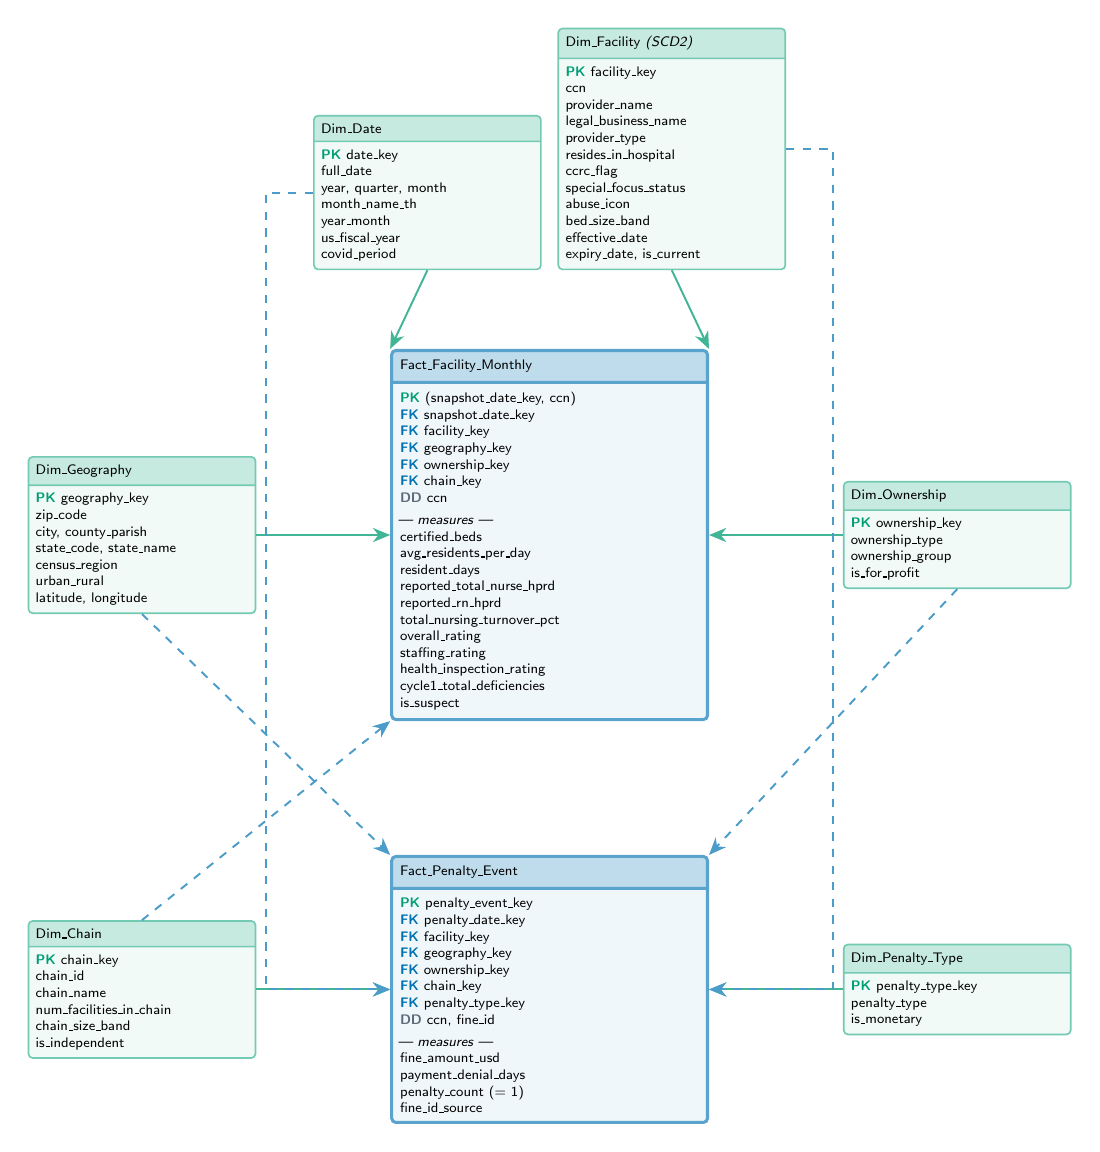
\begin{tikzpicture}[node distance=7mm]

% ---- FACT 1 ----
\node[factn] (f1) {
  Fact\_Facility\_Monthly
  \nodepart{two}
  \PK\ (snapshot\_date\_key, ccn)\\
  \FK\ snapshot\_date\_key\\
  \FK\ facility\_key\\
  \FK\ geography\_key\\
  \FK\ ownership\_key\\
  \FK\ chain\_key\\
  \DD\ ccn\\[2pt]
  \textit{— measures —}\\
  certified\_beds\\
  avg\_residents\_per\_day\\
  resident\_days\\
  reported\_total\_nurse\_hprd\\
  reported\_rn\_hprd\\
  total\_nursing\_turnover\_pct\\
  overall\_rating\\
  staffing\_rating\\
  health\_inspection\_rating\\
  cycle1\_total\_deficiencies\\
  is\_suspect
};

% ---- FACT 2 ----
\node[factn, below=17mm of f1] (f2) {
  Fact\_Penalty\_Event
  \nodepart{two}
  \PK\ penalty\_event\_key\\
  \FK\ penalty\_date\_key\\
  \FK\ facility\_key\\
  \FK\ geography\_key\\
  \FK\ ownership\_key\\
  \FK\ chain\_key\\
  \FK\ penalty\_type\_key\\
  \DD\ ccn, fine\_id\\[2pt]
  \textit{— measures —}\\
  fine\_amount\_usd\\
  payment\_denial\_days\\
  penalty\_count (= 1)\\
  fine\_id\_source
};

% ---- LEFT ----
\node[dimn, left=17mm of f1] (dgeo) {
  Dim\_Geography
  \nodepart{two}
  \PK\ geography\_key\\
  zip\_code\\
  city, county\_parish\\
  state\_code, state\_name\\
  census\_region\\
  urban\_rural\\
  latitude, longitude
};
\node[dimn, left=17mm of f2] (dchain) {
  Dim\_Chain
  \nodepart{two}
  \PK\ chain\_key\\
  chain\_id\\
  chain\_name\\
  num\_facilities\_in\_chain\\
  chain\_size\_band\\
  is\_independent
};

% ---- RIGHT ----
\node[dimn, right=17mm of f1] (down) {
  Dim\_Ownership
  \nodepart{two}
  \PK\ ownership\_key\\
  ownership\_type\\
  ownership\_group\\
  is\_for\_profit
};
\node[dimn, right=17mm of f2] (dpen) {
  Dim\_Penalty\_Type
  \nodepart{two}
  \PK\ penalty\_type\_key\\
  penalty\_type\\
  is\_monetary
};

% ---- TOP ----
\node[dimn, above left=10mm and 1mm of f1.north] (ddate) {
  Dim\_Date
  \nodepart{two}
  \PK\ date\_key\\
  full\_date\\
  year, quarter, month\\
  month\_name\_th\\
  year\_month\\
  us\_fiscal\_year\\
  covid\_period
};
\node[dimn, above right=10mm and 1mm of f1.north] (dfac) {
  Dim\_Facility \textit{(SCD2)}
  \nodepart{two}
  \PK\ facility\_key\\
  ccn\\
  provider\_name\\
  legal\_business\_name\\
  provider\_type\\
  resides\_in\_hospital\\
  ccrc\_flag\\
  special\_focus\_status\\
  abuse\_icon\\
  bed\_size\_band\\
  effective\_date\\
  expiry\_date, is\_current
};

% ---- edges ----
\draw[ar, draw=dw!75] (ddate.south) -- (f1.north west);
\draw[ar, draw=dw!75] (dfac.south)  -- (f1.north east);
\draw[ar, draw=dw!75] (dgeo.east)   -- (f1.west);
\draw[ar, draw=dw!75] (down.west)   -- (f1.east);
\draw[ar, draw=dw!75] (dchain.east) -- (f2.west);
\draw[ar, draw=dw!75] (dpen.west)   -- (f2.east);

% conformed dimensions = dashed
\draw[ar, draw=src!70, dashed] (dgeo.south) -- (f2.north west);
\draw[ar, draw=src!70, dashed] (down.south) -- (f2.north east);
\draw[ar, draw=src!70, dashed] (dfac.east) -- ++(6mm,0) |- (f2.east);
\draw[ar, draw=src!70, dashed] (ddate.west) -- ++(-6mm,0) |- (f2.west);
\draw[ar, draw=src!70, dashed] (dchain.north) -- (f1.south west);

\end{tikzpicture}
\end{adjustbox}
\caption{The star schema: two fact tables, six dimensions. Solid green edges are
a fact's own relationships; dashed blue edges mark conformed dimensions shared
by both facts. \PK\ primary key, \FK\ foreign key, \DD\ degenerate dimension —
the source system's own identifier, kept in the fact table itself. Stacking the
facts vertically keeps the diagram on one portrait page and makes the shared
dimensions obvious: they are the ones with edges going both up and down.}
\end{figure}

\begin{warnbox}[title={Fact 1 is keyed on \code{ccn}, not on \code{facility\_key}}]
\code{facility\_key} is an SCD2 surrogate, so one facility owns several values
of it. A primary key built on it would legitimately accept two rows for the
same facility in the same period, as long as a version boundary fell between
them — which is exactly the duplicate the grain forbids. \code{ccn} is the
identity that survives versioning, so it is kept in the fact table as a
degenerate dimension and used in the key.
\end{warnbox}

\subsection{Slowly changing dimension, type 2}

\code{Dim\_Facility} tracks history with \code{effective\_date} /
\code{expiry\_date} / \code{is\_current}. \textbf{15{,}983} facilities are
represented by \textbf{24{,}779} versions, of which 15{,}982 are current.
Because \code{facility\_key} is not one-to-one with \code{ccn}, every join from
a fact to this dimension must select the version whose validity window contains
the fact's date. That rule lives in exactly one function,
\code{facts.lookup\_facility\_key()}, and is never rewritten inline.

Two refinements were needed once the rule met real data. Version comparison
ignores columns unknown on either side, because going from unknown to known (a
column such as \code{abuse\_icon}, absent in 2019) is late data, not a change of
state — without this, crossing the 2019$\to$2026 boundary would have opened a
spurious version for all 14{,}300 facilities at once. And a fact older than the
earliest known version attaches to that version rather than to \code{Unknown},
since penalties reach back further than the oldest snapshot loaded.

\subsection{What was actually built}

Table~\ref{tab:rows} is the live content of the warehouse, read out of
\code{eldercare.duckdb} while this report was written.

\begin{table}[htbp]\centering\small
\begin{tabular}{L{4.6cm} R{2.2cm} L{8.2cm}}
\toprule
\sansall\bfseries Table & \sansall\bfseries Rows & \sansall\bfseries Notes \\
\midrule
\code{Dim\_Date} & 24{,}838 & 1960-01-01 to 2027-12-31, plus \code{date\_key = -1} \\
\code{Dim\_Facility} & 24{,}779 & 15{,}983 facilities, SCD2 \\
\code{Dim\_Geography} & 9{,}726 & (ZIP, city, state) grain, 53 states/territories \\
\code{Dim\_Ownership} & 14 & 13 types collapsed into 3 groups \\
\code{Dim\_Chain} & 639 & 637 chains, plus \code{Independent} and \code{Unknown} \\
\code{Dim\_Penalty\_Type} & 3 & Fine, Payment Denial, Unknown \\
\code{Fact\_Facility\_Monthly} & 44{,}966 & 3 periods (15{,}578 / 14{,}695 / 14{,}693); 96 rows flagged \\
\code{Fact\_Penalty\_Event} & 24{,}969 & 20{,}890 fines worth \$697.8M; 4{,}079 denials, 114{,}320 days \\
\code{Ref\_State\_Population} & 255 & (state, year) grain — deliberately not on Dim\_Geography \\
\code{etl\_run\_log} & 701 & Every quality rule's output \\
\bottomrule
\end{tabular}
\caption{Live contents of \code{eldercare.duckdb}, queried read-only for this
report. Eight modelled tables plus two supporting tables, and ten views.}
\label{tab:rows}
\end{table}

Every dimension carries a \code{key = -1} ``Unknown'' row so that no fact ever
holds a null foreign key — a null foreign key drops rows silently on join.
\code{Dim\_Chain} additionally distinguishes \code{Independent (no chain)}
(\code{chain\_key = 0}) from \code{Unknown} (\code{-1}), because a blank in 2026
means ``confirmed not in a chain'' whereas 2019 had no chain column at all.

\subsection{The semantic layer}

Ten views in \code{views.sql} define M1--M10 once. \textbf{Dashboards query the
views, not the fact tables.} The reason is not tidiness: three of the ten
measures give a plausible-looking wrong answer if computed naively, and the
wrong answer is convincing enough to survive a presentation. M1 must be a ratio
of sums; M3 and M4 must be weighted by M2, or a 20-bed home outvotes a 300-bed
home; M9 must not join the two facts directly.

% =====================================================================
\section{The ETL process}
% =====================================================================

\begin{figure}[tbp]
\centering
\begin{adjustbox}{max width=\linewidth}
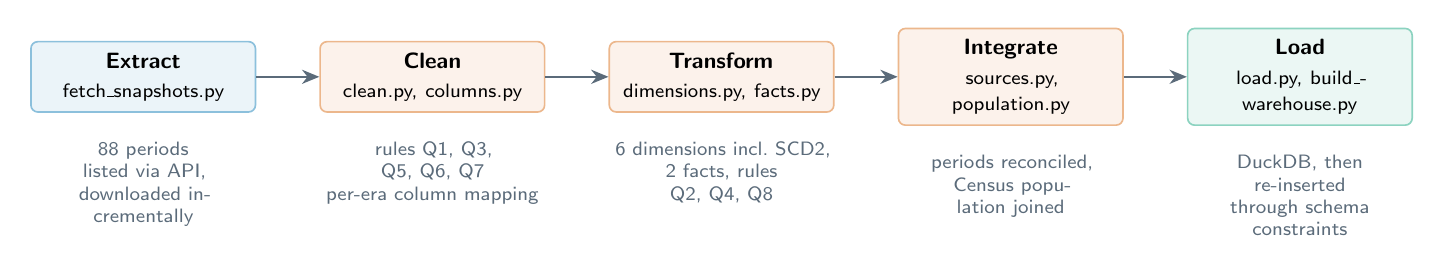
\begin{tikzpicture}[node distance=6mm]
\node[srcb, text width=25mm] (e) {\textbf{Extract}\\[1pt]
  \scriptsize fetch\_snapshots.py};
\node[etlb, text width=25mm, right=8mm of e] (c) {\textbf{Clean}\\[1pt]
  \scriptsize clean.py, columns.py};
\node[etlb, text width=25mm, right=8mm of c] (t) {\textbf{Transform}\\[1pt]
  \scriptsize dimensions.py, facts.py};
\node[etlb, text width=25mm, right=8mm of t] (i) {\textbf{Integrate}\\[1pt]
  \scriptsize sources.py, population.py};
\node[dwb, text width=25mm, right=8mm of i] (l) {\textbf{Load}\\[1pt]
  \scriptsize load.py, build\_warehouse.py};

\draw[ar] (e) -- (c);
\draw[ar] (c) -- (t);
\draw[ar] (t) -- (i);
\draw[ar] (i) -- (l);

\node[lbl, below=2.5mm of e, text width=27mm] {88 periods listed via API,\\downloaded incrementally};
\node[lbl, below=2.5mm of c, text width=27mm] {rules Q1, Q3, Q5, Q6, Q7\\per-era column mapping};
\node[lbl, below=2.5mm of t, text width=27mm] {6 dimensions incl.\ SCD2,\\2 facts, rules Q2, Q4, Q8};
\node[lbl, below=2.5mm of i, text width=27mm] {periods reconciled,\\Census population joined};
\node[lbl, below=2.5mm of l, text width=27mm] {DuckDB, then re-inserted\\through schema constraints};
\end{tikzpicture}
\end{adjustbox}
\caption{The five ETL stages and the module that owns each. Blue is the source
stage, orange the transformation stages, green the warehouse — the same colour
language as the star schema and the dashboard charts.}
\label{fig:etl}
\end{figure}

Figure~\ref{fig:etl} shows the five stages and which module owns each.

\textbf{Tools.} Python 3 with pandas for all transformation, DuckDB as a
single-file warehouse, Streamlit with matplotlib for the dashboard. The whole
pipeline is five commands and needs no manual data editing at any step.

\subsection{How each source is brought in}

\code{fetch\_snapshots.py} calls the CMS archive API, which returns 96 entries:
88 of type \code{theme} (real periods) and 8 of type \code{annual\_theme}
(yearly bundles that duplicate them). Only the former are kept. Downloads are
\textbf{incremental} — a period already on disk is skipped — and only the six
needed CSVs are extracted from each archive. Population comes from
\code{population.py}, which prefers the Census ACS API when
\code{CENSUS\_API\_KEY} is set and otherwise falls back to a static estimates
CSV; either path lands in the same shape and the run log records which was used.

\subsection{How the sources are connected}

\code{ccn} is the join key throughout, which is why the leading-zero rule (Q1)
is enforced at read time rather than patched later. Facts join to
\code{Dim\_Facility} through the SCD2 lookup described in section~5.3. Two
periods, \code{2026-07-29} and \code{2026-08-06}, share a processing date of
\code{2026-07-01}; without reconciliation the primary key of Fact 1 would
collide immediately, so republished periods are collapsed keeping the later
edition. Population is joined on state, at (state, year) grain, and deliberately
not stored on \code{Dim\_Geography} — that table is at (ZIP, city, state) grain,
so writing a state population onto every ZIP row would let a careless
\code{SUM} multiply Texas by its number of ZIP codes.

\subsection{Checking before and after load}

\begin{goodbox}[title={Verification results, all re-run for this report}]
\begin{tabular}{@{}L{5.0cm} L{7.4cm} R{2.2cm}@{}}
\toprule
\sansall\bfseries Suite & \sansall\bfseries Checks & \sansall\bfseries Result \\
\midrule
\code{verify\_dims.py} & Six dimensions, including SCD2 integrity & 22 / 22 \\
\code{verify\_facts.py} & Both facts, including reconciliation with CMS & 22 / 22 \\
\code{verify\_dashboard.py} & Dashboard measures vs.\ warehouse views, to 1e-9 & 56 / 56 \\
\code{test\_dashboard.py} & The app run under 11 real filter combinations & 11 / 11 \\
\bottomrule
\end{tabular}

\vspace{0.5em}
\textbf{The strongest single piece of evidence} is not any of these suites,
because a suite written by the same authors as the pipeline can agree with it
and both be wrong. It is a reconciliation against a number CMS computed
independently: restricting \code{Fact\_Penalty\_Event} to the fines present in
the June 2026 penalties file and summing per facility reproduces the CMS
\code{Total Amount of Fines in Dollars} column for \textbf{all 6{,}563
facilities}, totalling \textbf{\$459{,}054{,}863}, matching to the dollar.
\end{goodbox}

Checking happens at three levels. \textbf{Before load}, \code{load.py}
validates primary keys, foreign keys and SCD2 windows on the in-memory frames.
\textbf{At load}, \code{build_warehouse.py} copies each table aside, recreates
it empty from \code{schema.sql} with keys, uniqueness and \code{CHECK}
constraints, and re-inserts the data \emph{through} them — a bad row aborts the
run and the previous state is restored, so the insert \emph{is} the test rather
than a declaration about it. This matters because the ETL writes with
\code{CREATE OR REPLACE TABLE ... AS SELECT}, which keeps the data but discards
every contract, and a Python assertion does not travel inside a \code{.duckdb}
file handed to somebody else. The constraints were confirmed to bite: an
injected \code{facility_key = 88888888} was rejected as a foreign key violation
and \code{overall_rating = 9} as a \code{CHECK} violation. \textbf{After load},
the suites above query the database with SQL written independently of the code
that produced it.

\textbf{The pipeline is re-runnable.} Dimensions are rebuilt whole every time,
so no state survives between runs, and three consecutive builds produce
identical results. \code{run\_dims.py} deliberately drops the fact tables on
success: surrogate keys are handed out in row order, so rebuilding dimensions
from a different set of periods shifts them, and stale facts would still join —
to the wrong facility, silently. A missing table is an error you notice.

% =====================================================================
\section{The dashboard}
% =====================================================================

The dashboard is a Streamlit application reading the warehouse read-only.

\begin{table}[htbp]\centering\small
\begin{tabular}{L{6.4cm} R{2.4cm} R{2.4cm} L{3.6cm}}
\toprule
\sansall\bfseries Requirement & \sansall\bfseries Required &
\sansall\bfseries Delivered & \sansall\bfseries Where \\
\midrule
Measures summarising business performance & $\geq$ 3 & \textbf{10} & Header strip and tabs \\
Charts & $\geq$ 5 & \textbf{13} & All tabs \\
Time-based analysis & $\geq$ 1 & \textbf{2} & BQ5 cohort, BQ7 fines by year \\
Comparison of data & $\geq$ 1 & \textbf{2} & BQ2 ownership, BQ8 chain size \\
Filters / interactive controls & $\geq$ 2 & \textbf{5} & Period, state, ownership, chain size, suspect-row switch \\
Insights and recommendations & $\geq$ 5 & \textbf{8} & One per business question \\
\bottomrule
\end{tabular}
\caption{Compliance with the brief's dashboard requirements.
\code{verify\_dashboard.py} counts these \emph{from the code} rather than
asserting them from memory, so the table cannot quietly go out of date.}
\end{table}

\begin{figure}[tbp]
\centering
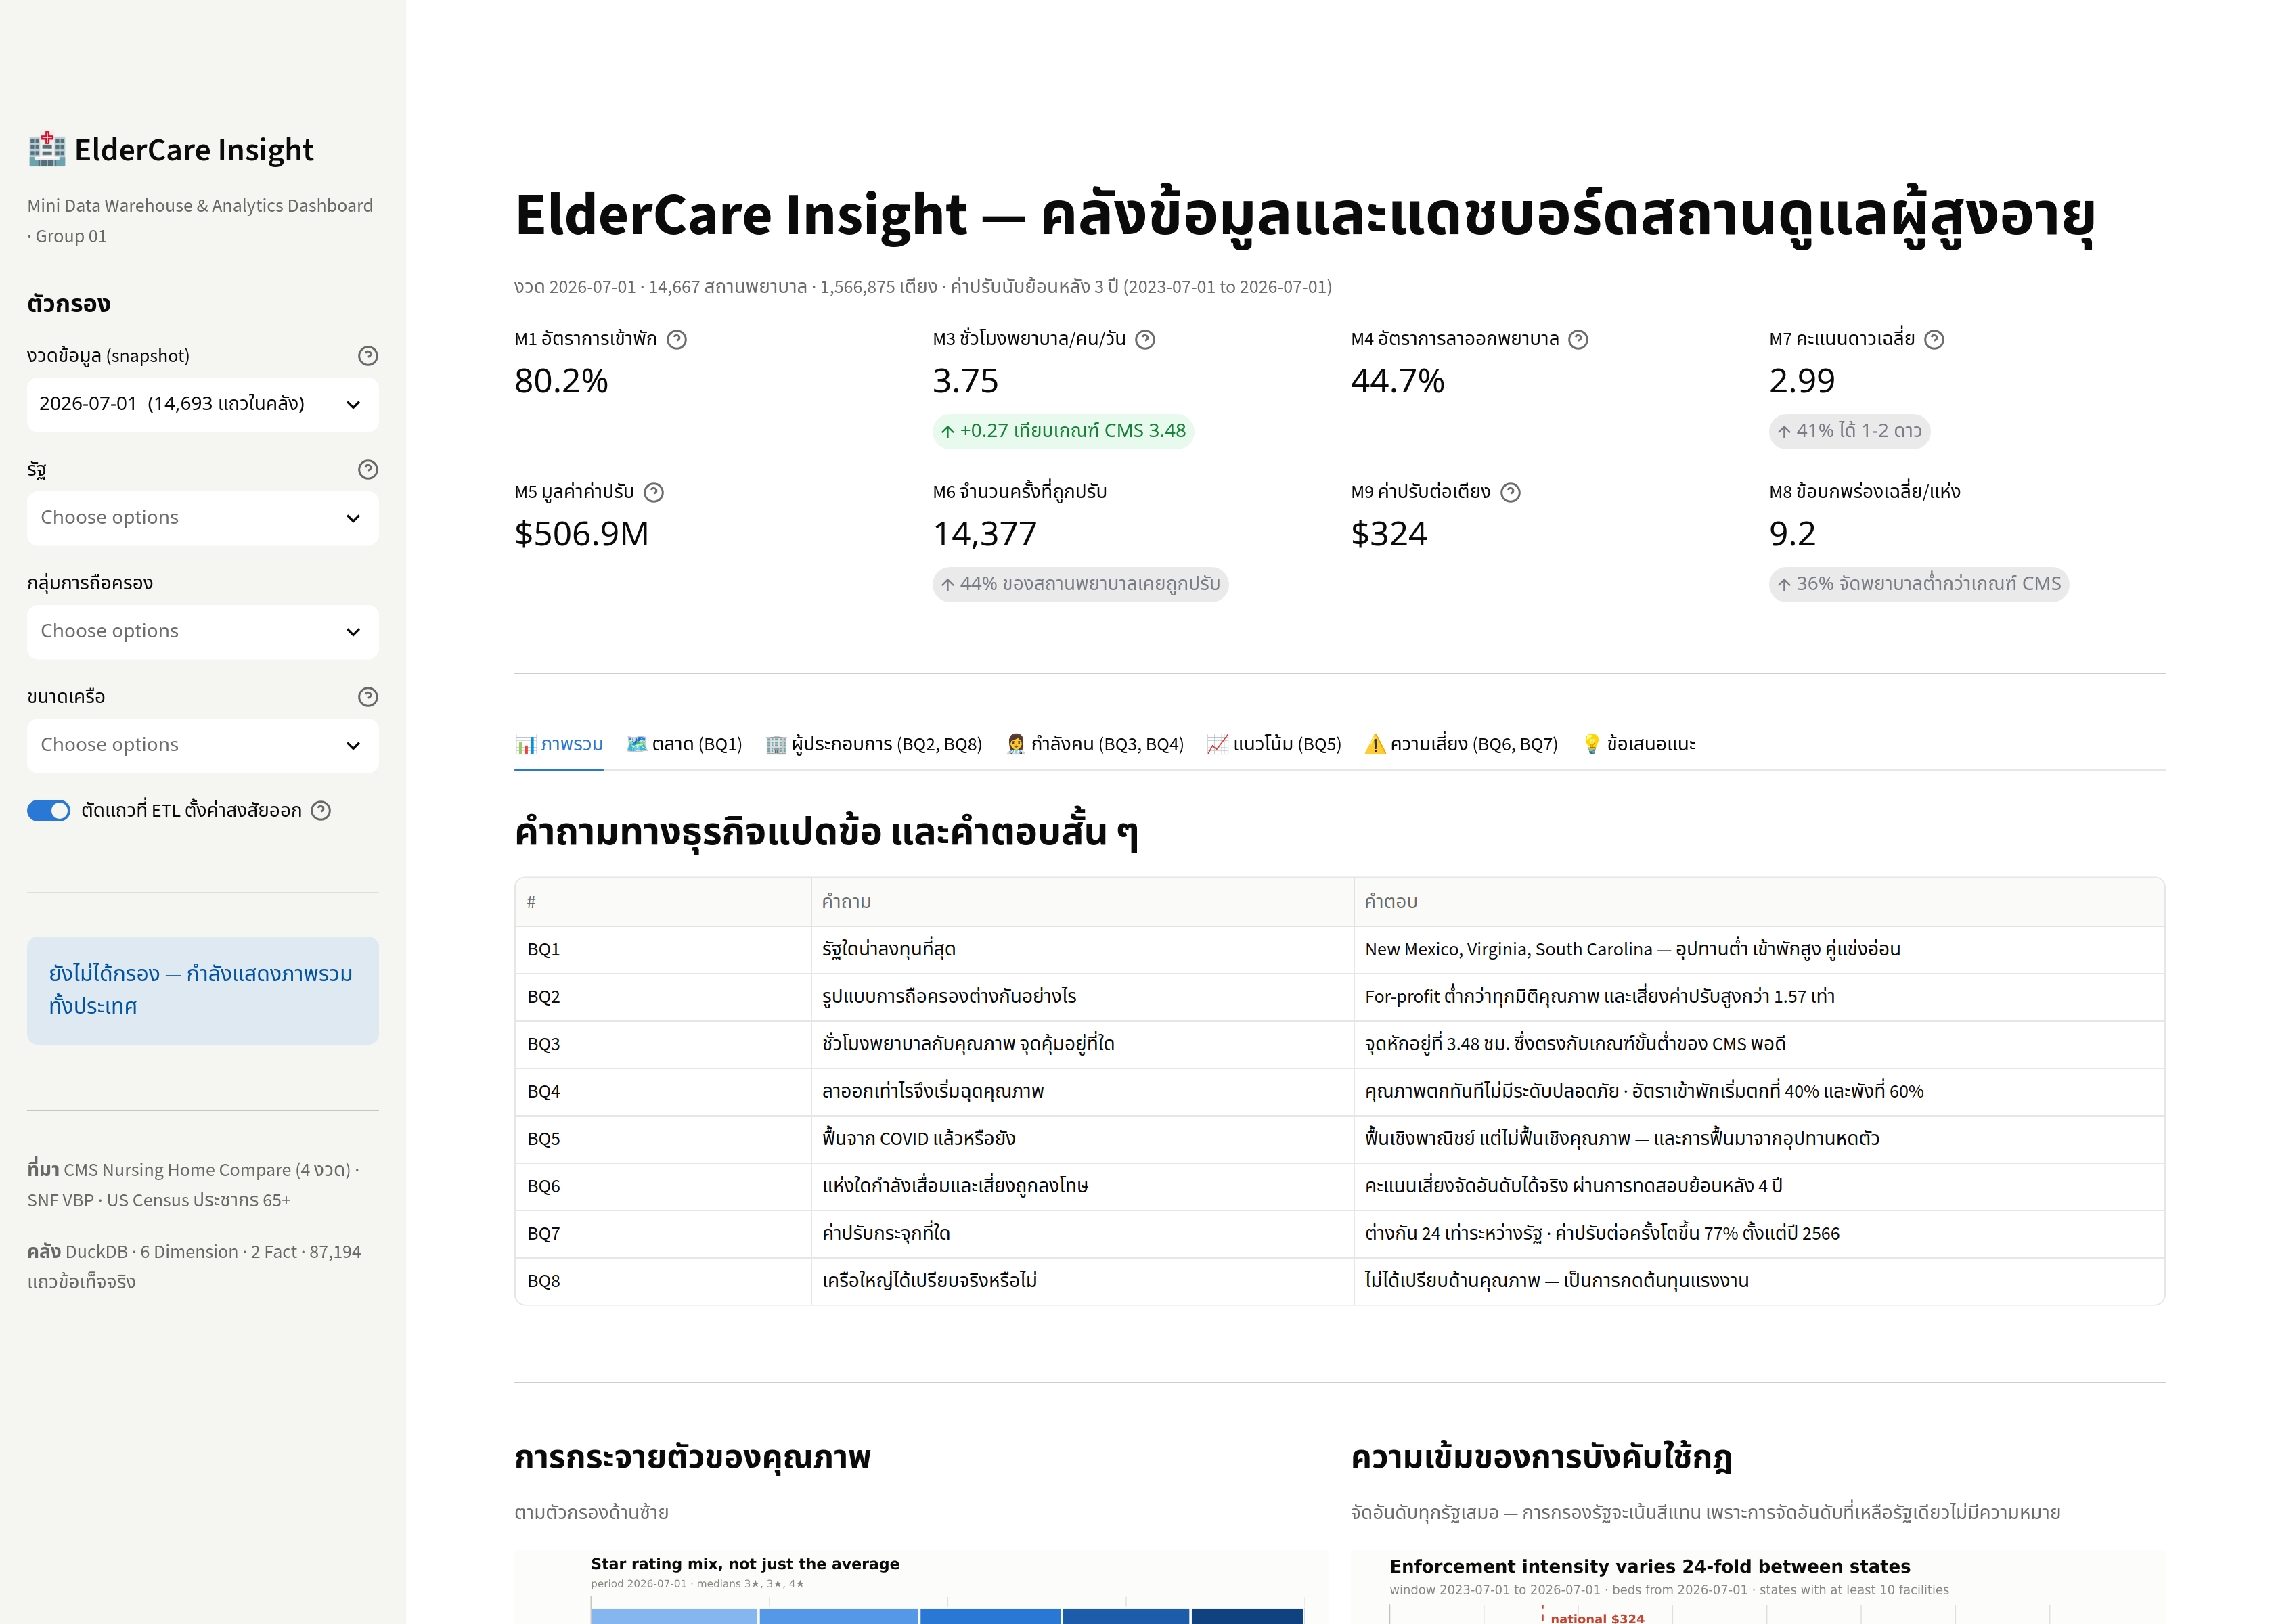
\includegraphics[width=0.96\linewidth]{01_overview}
\caption{The complete dashboard, unfiltered, showing the national position:
the measure strip across the top, and the eight business questions with their
one-line answers below. Interface labels are Thai because the intended audience
is Thai; the chart interiors are English. Tabs, left to right: Overview,
Market (BQ1), Operators (BQ2, BQ8), Workforce (BQ3, BQ4), Trend (BQ5), Risk
(BQ6, BQ7), Recommendations, Data quality.}
\end{figure}

\begin{figure}[tbp]
\centering
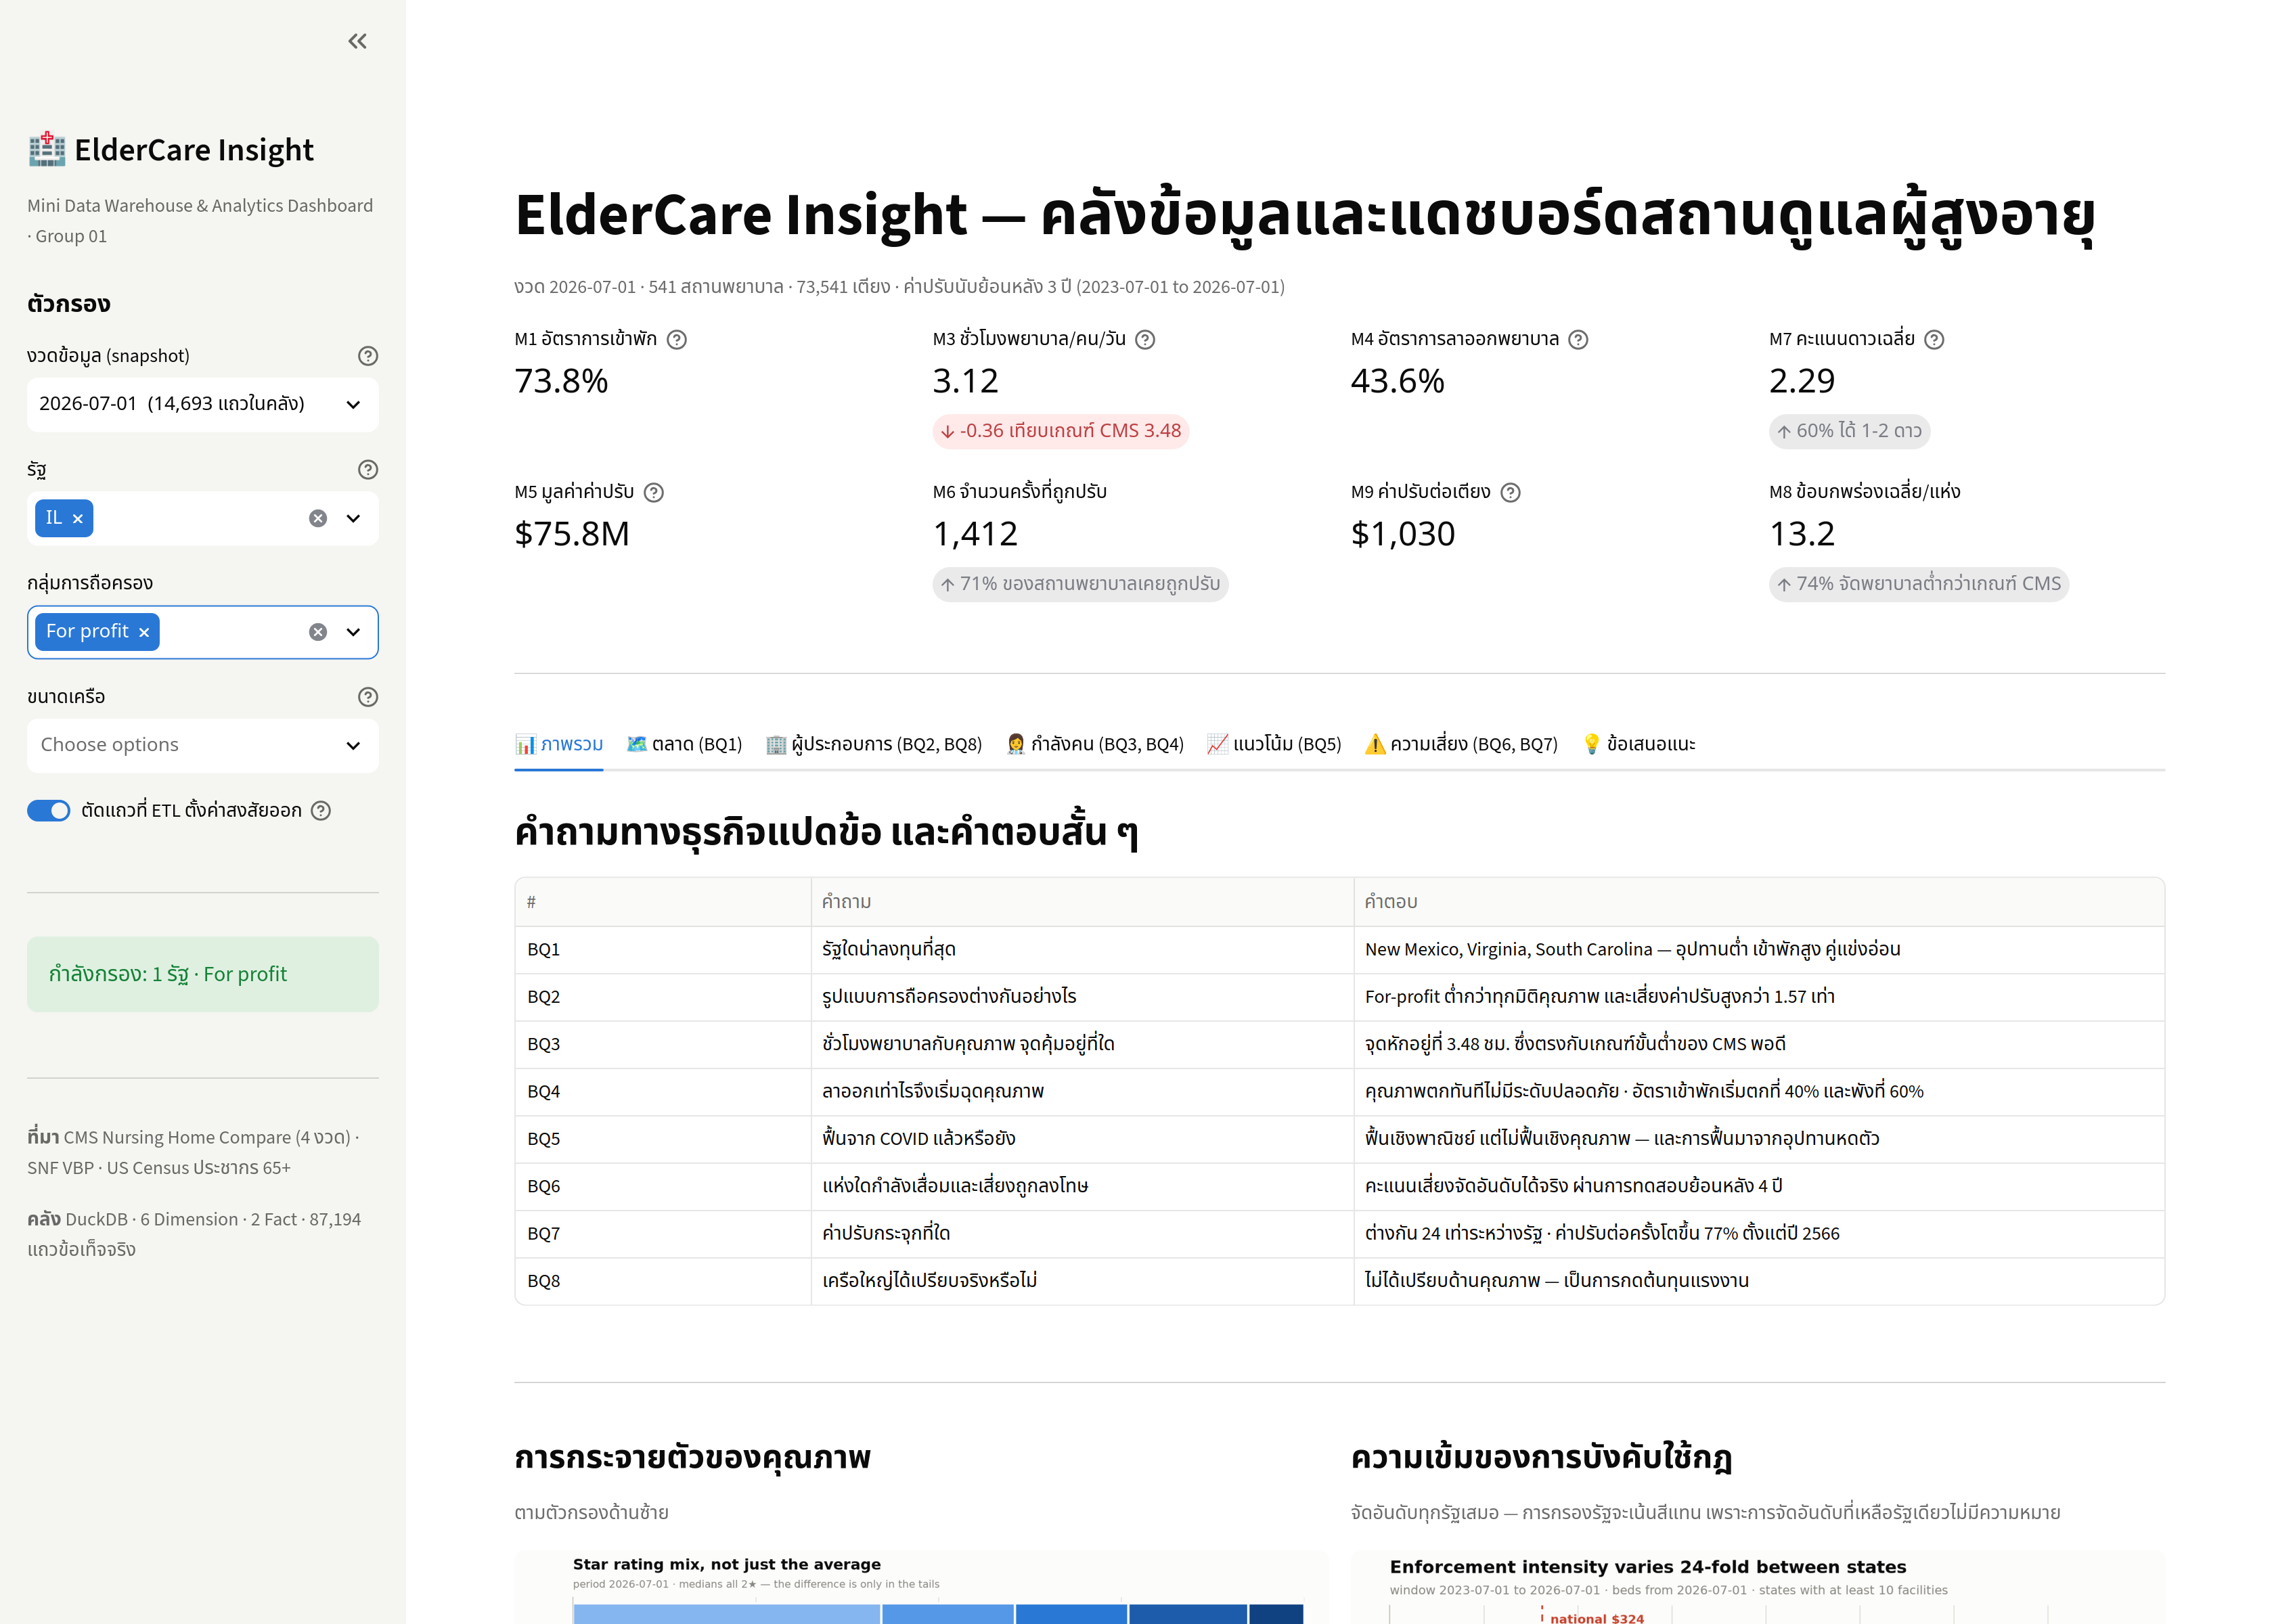
\includegraphics[width=0.96\linewidth]{08_filtered_IL_forprofit}
\caption{The same view after two filters are applied in the sidebar — state
\textbf{IL} and ownership group \textbf{For profit}. Every measure and every
chart recomputes; the occupancy figure in the header moves, which is how the
capture is validated. \code{make\_screenshots.py} reads a headline measure
before and after applying the filter and \textbf{refuses to save the image if
the value did not change}, so this figure cannot claim an interaction that
never happened.}
\end{figure}

\begin{keybox}[title={Three design rules the dashboard follows}]
\textbf{Read the views, never the fact tables.} A dashboard that reaches past
the semantic layer and writes its own \code{AVG(residents/beds)} reports
occupancy about 1.7 points too high with no error. Where a filter makes a
pre-aggregated view unusable, the formula is repeated in
\code{queries.MEASURES\_SQL} — and that duplication is \emph{guarded}, not
trusted: \code{verify\_dashboard.py} recomputes every measure through the
dashboard's own constant and asserts it matches the warehouse view to 1e-9.

\vspace{0.3em}
\textbf{Insights are computed at render time, not written into the page.} A
hard-coded insight is a sentence that was true of one dataset and has nothing
tying it to the chart above it. Here the text and the chart read the same
numbers in the same request, so they cannot contradict each other, and moving a
filter recomputes the conclusion. Each insight carries an evidence-strength
marker and an explicit caveat line.

\vspace{0.3em}
\textbf{Show what is missing rather than hiding it.} A data-quality tab, fed
live from \code{etl\_run\_log}, states the limitations of section~11 on screen
rather than only in this report.
\end{keybox}

A second implementation of the same dashboard exists in the repository
(\code{app.py}, using Plotly and reading the SQL view layer directly). Both
answer BQ1--BQ8 and both pass their test suites; the screenshots in this report
are of \code{app\_mpl.py}.

% =====================================================================
\section{Business insights and recommendations}
% =====================================================================

All figures below are for period 2026-07-01, with the penalty window
2023-07-01 to 2026-07-01, and come from \code{queries\_mpl.py} — the same module
the dashboard calls, so the report and the screen agree by construction rather
than by coincidence.

\subsection{BQ1 — where to expand}

New Mexico, Virginia and South Carolina rank highest: all three combine
below-average supply, above-average occupancy and weak incumbent quality.
Nationally there are 25.6 beds per 1{,}000 people aged 65+, occupancy is 80.2\%
and the average competitor scores 2.99 stars; New Mexico sits at 16.1 beds,
83.4\% and 2.85. \textbf{Recommendation:} shortlist these three, and avoid
Arkansas, Indiana and Iowa, where more than 40 beds per 1{,}000 elderly coexist
with occupancy in the 70s — adding capacity there only takes residents from
existing homes.

\subsection{BQ2 — ownership matters, and in one direction}

\begin{table}[htbp]\centering\small
\begin{tabular}{L{4.4cm} R{2.6cm} R{2.6cm} R{2.6cm}}
\toprule
& \sansall\bfseries For profit & \sansall\bfseries Non profit &
\sansall\bfseries Government \\
\midrule
Facilities & 10{,}845 & 2{,}875 & 947 \\
Average star rating & \textbf{2.80} & 3.57 & 3.28 \\
Nurse hours per resident-day & \textbf{3.62} & 4.21 & 4.17 \\
Turnover & \textbf{45.8\%} & 40.4\% & 42.4\% \\
Fines per bed & \textbf{\$351} & \$224 & \$250 \\
Ever fined & \textbf{48.7\%} & 37.1\% & 43.7\% \\
\bottomrule
\end{tabular}
\end{table}

For-profit facilities trail on every quality dimension and carry 1.57 times the
penalty exposure per bed of non-profits. \textbf{Recommendation:} in
acquisition diligence, treat for-profit ownership as a risk factor that has to
be priced, not as a neutral attribute — and budget for the staffing gap, since
the 0.77-star difference tracks a 16\% difference in nurse hours.

\subsection{BQ3 — the staffing break-even is 3.48 hours}

\begin{figure}[tbp]
\centering
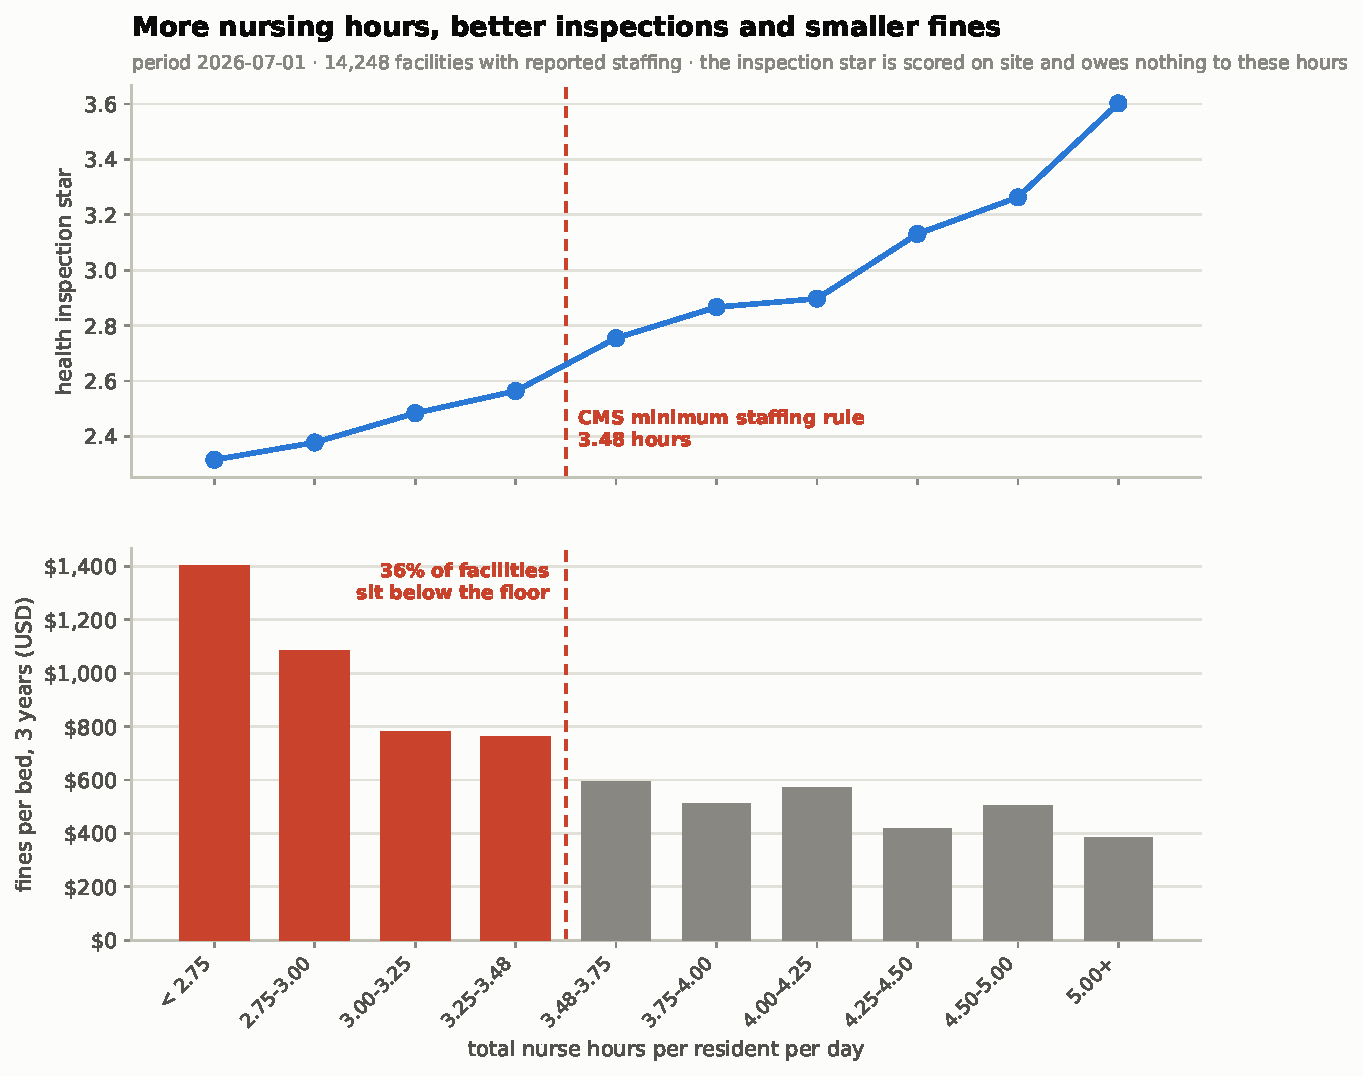
\includegraphics[width=0.74\linewidth]{bq3_staffing_gradient}
\caption{Health-inspection stars and fines per bed against nurse hours per
resident-day. The break-even sits exactly at the CMS minimum of 3.48 hours, and
the fine curve flattens above roughly 3.75.}
\end{figure}

Below 3.48 hours, fines per bed run \$404 against \$268 above it — 1.51 times
higher — and 52.6\% of facilities have been fined against 39.7\%. Above roughly
3.75 hours the fine curve is flat (\$289, \$264, \$283 across successive bands),
so extra hours still buy stars but no longer buy risk reduction.
\textbf{Recommendation:} 36\% of facilities (5{,}134) are still below the
threshold; the next staffing dollar belongs to them, not to topping up homes
that already clear it.

The conclusion rests on health-inspection stars and fines rather than the
overall rating, because CMS feeds nurse hours into the staffing star, which is
itself a component of the overall rating — plotting hours against the overall
score would be partly circular. The gradient also holds inside all three
ownership groups.

\subsection{BQ4 — two different thresholds for two different readers}

Quality has \emph{no} safe level of turnover: the rating falls from the very
first band and keeps falling, roughly 0.2 stars for every 5 points. Occupancy
behaves differently — flat near 83.5\% below 40\%, then losing 1.57 points
immediately in the 40--45\% band and collapsing to 71.7\% above 65\%. The
national average is 44.7\%. Retention is also an independent lever, not a shadow
of thin staffing: even in the best-staffed quartile, moving from under 40\% to
over 60\% turnover costs 1.34 stars — \emph{more} than the same move costs in
the thinnest-staffed quartile. \textbf{Recommendation:} HR should treat any
figure above zero as worth attacking, while the CFO should defend the 40\% line,
because that is where the money is; retention programmes are cheaper than
permanent headcount and the evidence says they work independently.

\subsection{BQ5 — a commercial recovery, not a clinical one}

Measured on the same 14{,}231 facilities open in both periods, occupancy rose
79.8\%~$\to$~80.2\% while the average rating fell 3.36~$\to$~2.97 and
deficiencies rose 23.7\%. The recovery is also not what it appears:
\textbf{1{,}282 facilities (8.25\%) closed, taking 98{,}725 beds with them}, and
the ones that closed had 64.9\% occupancy against 79.8\% for survivors.
Nationally beds fell 5.1\% while residents fell 3.5\% — \textbf{the denominator
left the market, so the ratio improved}. \textbf{Recommendation:} do not read
recovering occupancy as returning demand. Capacity decisions should be made on
state-level demand, not the national ratio.

\subsection{BQ6 — a risk score that survives a four-year backtest}

A five-component score (Special Focus status, 1--2 stars, prior heavy fines,
high deficiencies, staffing below the CMS minimum) assigned from the January
2019 data predicts outcomes more than four years later. It rises monotonically
on every outcome column: facilities scoring 0 were fined 35.6\% of the time and
averaged \$215 per bed; those scoring 6 were fined 59.5\% of the time at \$550
per bed. The high-risk group carries 1.29$\times$ the penalty rate and
1.52$\times$ the penalty value. \textbf{The finding that matters more than the
multiplier: facilities that scored 6 in 2019 still average only 2.21 stars seven
years later.} \textbf{Recommendation:} risk is persistent, not transient — any
acquisition of a flagged facility needs a turnaround budget attached, not an
assumption of mean reversion. The weights are deliberately small integers and
every component is shown on screen, because a COO who cannot see why a home is
on the list cannot act on it.

\subsection{BQ7 — a 24-fold spread under one federal rulebook}

\begin{figure}[tbp]
\centering
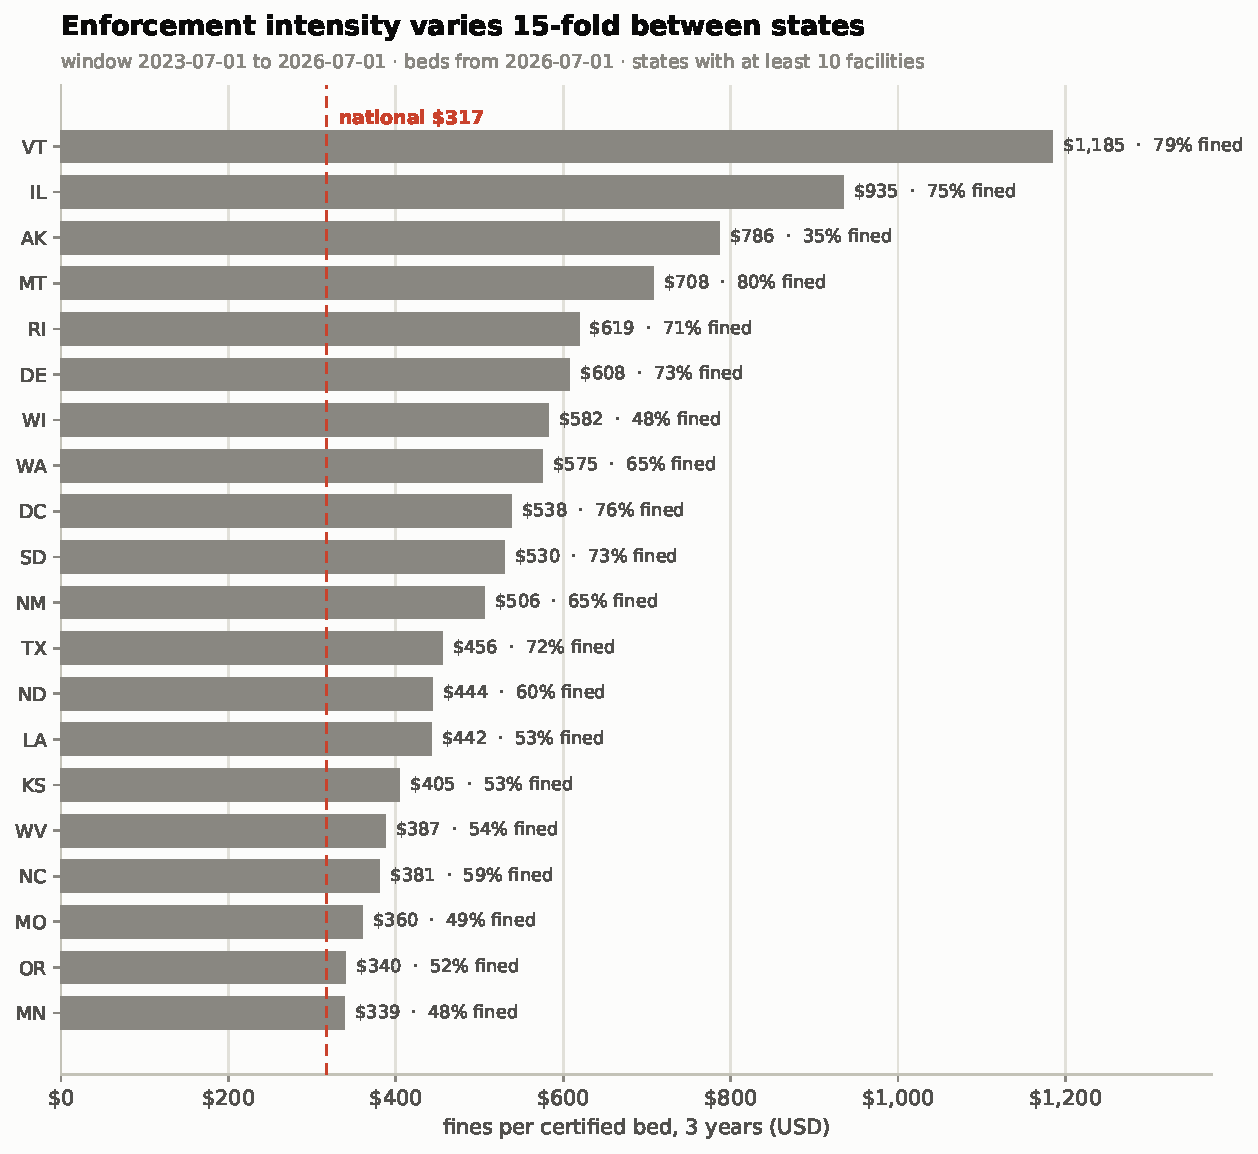
\includegraphics[width=0.64\linewidth]{bq7_state_enforcement}
\caption{Fines per certified bed by state over the three-year window.}
\end{figure}

Vermont levies \$1{,}364 per bed and Indiana \$57 — a 24-fold difference under
the same federal rules, against a national \$324. Five states (IL, TX, CA, OH,
FL) account for 43.9\% of all fines on 31.8\% of the beds. \textbf{Illinois is
the case to watch}, being both the largest exposure (\$81.7M) and the third
harshest per bed (\$960). The pattern is also changing over time: between 2023
and 2025 the average fine per event rose 76.7\% while the number of events fell
19.2\% — from ``often and small'' to ``rarely and hard''.
\textbf{Recommendation:} weight compliance spend by state, not by facility
count, and model penalty exposure as a small number of large events.

\subsection{BQ8 — scale buys occupancy, not care}

Independent homes average 4.09 nurse hours and 41.6\% turnover; chains of 50+
average 3.53 hours and 46.2\%, and score 0.32 stars lower. The obvious objection
is that large chains are almost all for-profit, so this might just be BQ2 under
another name. It is not: \textbf{nurse hours fall at every step of chain size
inside all three ownership groups} — for-profit 3.75$\to$3.54, non-profit
4.38$\to$3.47, government 4.56$\to$3.34. What scale genuinely delivers is
commercial, not clinical: occupancy is 1.6 points higher.
\textbf{Recommendation:} do not pay a quality premium for scale in an
acquisition; price the occupancy advantage and budget separately for the
staffing deficit that comes with it.

% =====================================================================
\section{Use of generative AI, and how its output was checked}
% =====================================================================

AI assistance was used throughout and is logged in
\code{05\_AI\_Usage\_Log/AI\_Usage\_Log.md}, which currently holds
\textbf{18 entries} against the required minimum of five. Each entry records the
prompt as actually typed, what the AI proposed, what was accepted, modified or
rejected, and — the field the group treats as decisive — how the output was
checked.

\textbf{What counts as checking} is fixed by group rule: running a command and
comparing to a known value, opening the real data file and counting rows
yourself, checking against the CMS data dictionary, or another member reading
the work and explaining it back. \textbf{What does not count:} ``it reads
sensibly'', ``the AI said it was confident'', ``asked again and got the same
answer'', and ``it ran without errors''.

Three examples where AI output was \textbf{not} taken as given:

\textbf{Rejected outright.} An AI review proposed adding
\code{payment\_denial\_start\_date} to the deduplication key for Fact 2. It does
discriminate better, but an attribute CMS can revise later must not sit in a key
— if the source corrects a date, the same penalty becomes a new row. The key was
kept narrow.

\textbf{Rejected on principle.} Two suggestions were refused for the same
reason — that hiding a defect is worse than showing it. Excluding
\code{is\_suspect} rows from the measure views by default contradicts the
flag-don't-delete rule, so the views report \code{suspect\_rows} alongside
instead; and hiding the BQ1 tab while M10 was incomplete would mean the reader
never learns of the gap, so the tab stays with a red box naming what is missing.

\textbf{Accepted as a finding, but verified independently first.} An AI-assisted
audit reported that the pipeline was dropping a third of its penalty rows. That
was not taken on trust: the group listed the extracted files for both periods,
re-counted the CSV rows with pandas (16{,}180 and 16{,}166), reproduced the
original total by hand ($8{,}789 + 16{,}180 + 16{,}166 = 41{,}135$), and traced
the regression to a specific commit with \code{git show}. Only then was it
recorded as a real defect — the one described in section~11. The same audit's
recommendation to revert the offending change was \emph{rejected}, because the
original reasoning was sound and the correct fix is narrower.

% =====================================================================
\section{Source files and how to reproduce this}
% =====================================================================

\textbf{Google Drive folder:} \underline{\hspace{7cm}} \quad (view access for
anyone with the link)

\textbf{Dashboard:} run locally with the commands below, or
\underline{\hspace{5cm}}

\begin{table}[htbp]\centering\small
\begin{tabular}{L{4.4cm} L{10.6cm}}
\toprule
\sansall\bfseries Folder & \sansall\bfseries Contents \\
\midrule
\code{01\_Raw\_Data/} & Download instructions; the data itself is not stored, but
  is always retrievable \\
\code{02\_ETL/} & The pipeline: extract, clean, transform, integrate, load, and two
  verification suites \\
\code{03\_Data\_Warehouse/} & \code{schema.sql}, \code{views.sql},
  \code{build\_warehouse.py}; the \code{.duckdb} file is rebuilt, not stored \\
\code{04\_Dashboard/} & Two Streamlit applications, chart layer, notebooks,
  figures, screenshots, tests \\
\code{05\_AI\_Usage\_Log/} & 18 logged entries \\
\code{06\_Report/} & This report, the full design document, and the eight
  business answers in long form \\
\bottomrule
\end{tabular}
\end{table}

Starting from an empty folder:

\begin{tcolorbox}[colback=wash, colframe=rule, boxrule=0.4pt, arc=1pt,
                  left=8pt, right=8pt, top=5pt, bottom=5pt]
\small\ttfamily
python -m pip install -r requirements.txt\\[2pt]
cd 02\_ETL\\
python fetch\_snapshots.py -{}-dates 2019-01-17 2026-06-24 2026-07-29 2026-08-06\\
python run\_dims.py \&\& python run\_facts.py \&\& python population.py\\
python verify\_dims.py \&\& python verify\_facts.py\\[2pt]
cd ../03\_Data\_Warehouse \&\& python build\_warehouse.py -{}-report\\[2pt]
cd ../04\_Dashboard \&\& python verify\_dashboard.py\\
streamlit run app\_mpl.py
\end{tcolorbox}

% =====================================================================
\section{Limitations}
% =====================================================================

Stated here rather than left for the reader to find.

\begin{enumerate}
\item \textbf{The penalty data is incomplete.} The deduplication rule collapses
  \code{2026-07-29} and \code{2026-08-06}, which share a processing date, by
  keeping the later edition — but that edition is the 3.5~MB partial archive
  with no penalties file, so 16{,}166 penalty rows go with it. Every
  fines-per-bed figure here is therefore slightly understated and the latest
  penalty in the warehouse is dated 2026-05-13, not 2026-07-01.
  \textbf{Comparisons between groups remain valid, because every group is
  missing the same two months}; absolute levels need this caveat attached. The
  fix is to deduplicate per file rather than per period. Note that
  \code{verify\_facts.py} still reports 22/22, having no check that every
  extracted file was read — a passing suite is not proof of completeness.
\item \textbf{Three time points, not a time series.} Snapshots exist for
  2019-01, 2026-06 and 2026-07, with a seven-year gap, so BQ5 is a matched
  cohort comparison between two endpoints rather than a trend: it says where the
  sector ended up, not when it bottomed out. The charts break the line across
  the gap instead of interpolating. For the same reason M9 compares across
  states within a year but not across years.
\item \textbf{Chain data exists only for 2026}, so BQ8 cannot distinguish
  ``chains degrade the homes they own'' from ``chains buy homes that were already
  weak''.
\item \textbf{Turnover exists only in the 2026 era}, so BQ4 is cross-sectional.
\item \textbf{Two population paths.} \code{Ref\_State\_Population} is populated
  and drives the BQ1 figures quoted here. The older
  \code{Dim\_Geography.pop\_65plus} column remains empty, so the
  \code{v\_market\_saturation} view — and the Plotly dashboard that reads it —
  still returns null for M10. Consolidating the view onto
  \code{Ref\_State\_Population} is outstanding work.
\item \textbf{The VBP source is extracted but not yet modelled}; a third fact at
  facility $\times$ fiscal-year grain is designed but not built.
\end{enumerate}

\vspace{0.6em}
\begin{keybox}[title={Data source and licence}]
Centers for Medicare \& Medicaid Services, \textit{Provider Data Catalog —
Nursing Homes}, \url{https://data.cms.gov/provider-data/archived-data/nursing-homes}.
United States government public data, free to use with attribution.
Population figures from the U.S. Census Bureau.
\end{keybox}

\end{document}
